\documentclass[letterpaper]{article}
    % General document formatting
    \usepackage[parfill]{parskip}
    \usepackage[utf8]{inputenc}
    \usepackage[margin=2cm]{geometry}
    
    % Related to math
    \usepackage{amsmath,amssymb,amsfonts,amsthm}
    \usepackage{tikz}

\begin{document}

\thispagestyle{empty}

\begin{center}
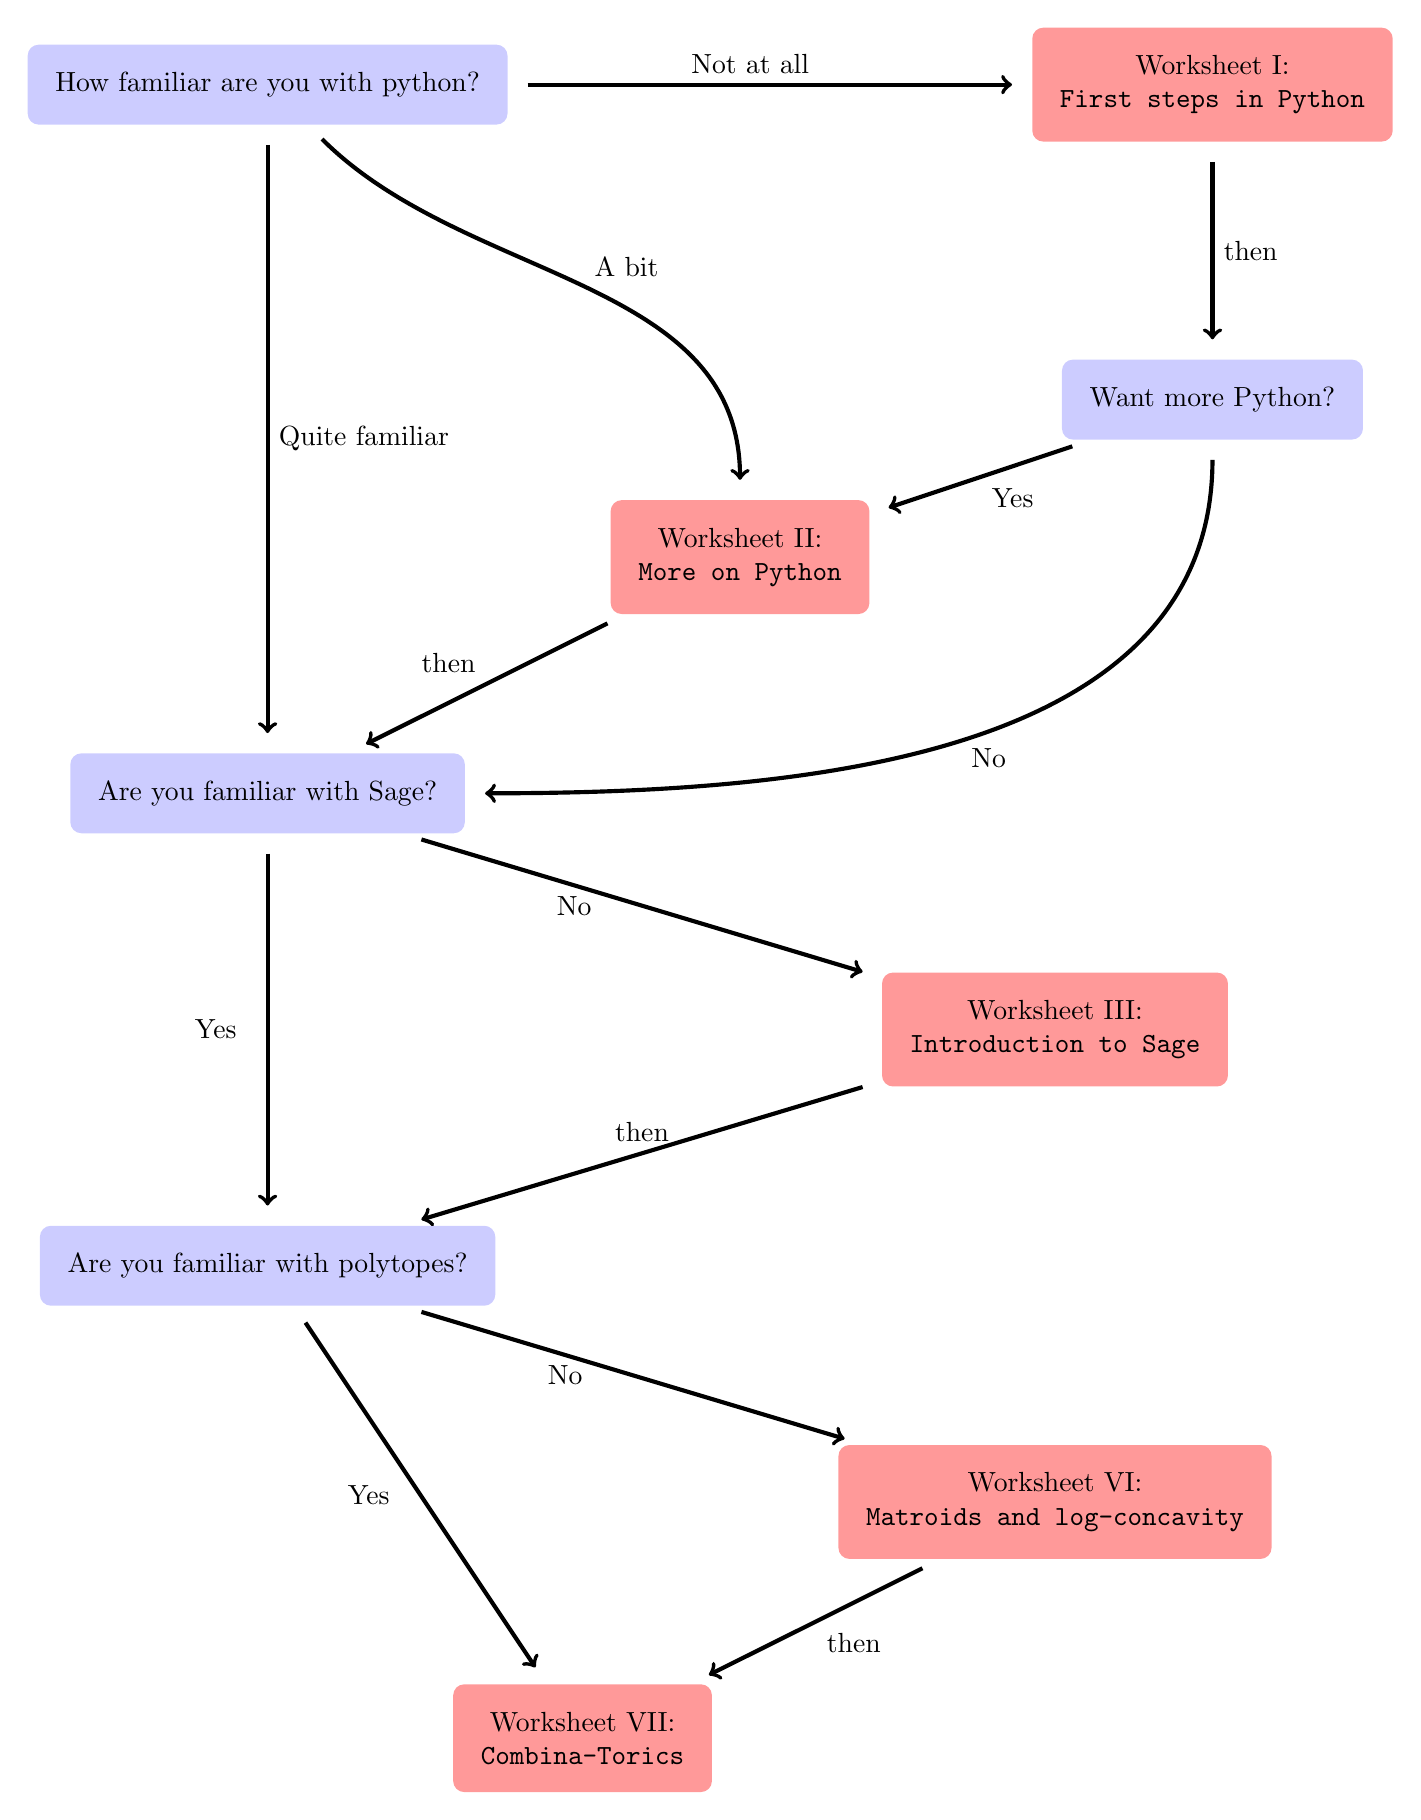
\begin{tikzpicture}[question/.style={fill=blue!20, align=center, rectangle, rounded corners,inner sep=10pt},
                    worksheet/.style={fill=red!40, align=center, rectangle, rounded corners,inner sep=10pt},
                    fleche/.style={line width=1.5pt, shorten >=0.25cm, shorten <=0.25cm}]

	\node[question] (FamPython) at (-6,10) {How familiar are you with python?};
	
	\node[worksheet] (BegPython) at (6,10) {Worksheet I:\\ \texttt{First steps in Python}};
	
	\node[worksheet] (RevPython) at (0,4) {Worksheet II:\\ \texttt{More on Python}};
	
	\node[question] (want) at (6,6) {Want more Python?};
	
	\node[question] (FamSage) at (-6,1) {Are you familiar with Sage?};
	
	\node[worksheet] (IntroSage) at (4,-2) {Worksheet III:\\ \texttt{Introduction to Sage}};
	
	\node[question] (FamPoly) at (-6,-5) {Are you familiar with polytopes?};
	
	\node[worksheet] (IntroPoly) at (4,-8) {Worksheet VI:\\ \texttt{Matroids and log-concavity}};
	
	\node[worksheet] (CourseProb) at (-2,-11) {Worksheet VII:\\ \texttt{Combina-Torics}};
	
	
	\path[->, fleche] (FamPython) edge  node[above, align=center] {Not at all\hspace{0.5cm}} (BegPython);
	
	\path[->, fleche,in=90,out=-45] (FamPython) edge  node[above right, align=center] {A bit} (RevPython);
	
	\path[->, fleche] (BegPython) edge node[right,align=center] {then} (want);	
	
	\path[->, fleche] (want) edge node[below right,align=center] {Yes} (RevPython);

	\path[->, fleche,out=270,in=0] (want) edge node[below right,align=center] {No} (FamSage);

	\path[->, fleche] (RevPython) edge node[above left,align=center] {then} (FamSage);	

	\path[->, fleche] (FamPython) edge  node[right, align=center] {Quite familiar} (FamSage);

	\path[->, fleche] (FamSage) edge node[left,align=center] {No\hspace{0.5cm}} (IntroSage);

	\path[->, fleche] (FamSage) edge node[left,align=center] {Yes\hspace{0.25cm}} (FamPoly);	
	\path[->, fleche] (IntroSage) edge node[above,align=center] {then} (FamPoly);	
	
	\path[->, fleche] (FamPoly) edge node[left,align=center] {No\hspace{0.5cm}} (IntroPoly);

	\path[->, fleche] (FamPoly) edge node[left,align=center] {Yes\hspace{0.25cm}} (CourseProb);	
	\path[->, fleche] (IntroPoly) edge node[below right,align=center] {then} (CourseProb);	
	
	
\end{tikzpicture}
\end{center}


\end{document}
